\documentclass[12pt]{article}
\usepackage[T2A]{fontenc}
\usepackage[utf8]{inputenc}
\usepackage[russian]{babel}
\usepackage{cmap}

\usepackage{hyphenat}

\usepackage{amsmath}
\usepackage{tabularx}
\usepackage{subcaption}
\usepackage{graphicx}
\usepackage{multicol}
\usepackage{floatrow}
\usepackage{indentfirst}

\usepackage{hyperref}
\usepackage{cleveref}
\hypersetup{
    colorlinks,
    citecolor=black,
    filecolor=black,
    linkcolor=black,
    urlcolor=black
}

\usepackage[dvipsnames]{xcolor}

\usepackage{amsthm,amssymb}

\usepackage{listings}

\newtheorem{lemma}{Лемма}
\newtheorem{theorem}{Теорема}
\newtheorem{remark}{Замечание}
\newtheorem{algorithm}{Алгоритм}
\newtheorem{technique}{Метод}
\renewcommand{\qedsymbol}{$\blacksquare$}

\usepackage[top=0.7in, bottom=1.1in, left=1in, right=1in]{geometry}

\title{3-расскрашиваемость графа}
\author{Крохалев Арсений}

\begin{document}
\maketitle

\section{Введение}
Существует много известных NP-полных задач, включая такие важные те\-о\-ре\-ти\-че\-ские проблемы в графе, как раскраски и независимые множества. Человечество до сих пор не знает, существовании полиномиальных алгоритмов для этих проблем, но это не устраняет необходимости их решения как можно эффективнее. Первый не тривиальный алгоритм был предложен Лаувером (Lawer, 1937), который работает за $O\left(1.4422^n\right)$. На сегодняшний день самый быстрый известный алгоритм работает за время $O\left(1.3289^n\right)$ и предложен Ричардом Бейгелем и Дэвидом Эппсштейном (Richard Beigel and David Eppstein, 2000)\cite{fast}.

В данной статье будет рассмотрен алгоритм Лаувера, а также доказательство вре\-ме\-ни работы $O\left(1.4422^n\right)$ и реализация на языке $\text{C++}$.

\section{Вспомогательные утверждения}
\subsection{Обозначения}
$\overline{a...b} = \left\{x \hookrightarrow x \in \mathbb{N} \wedge x \geq a \wedge x \leq b \right\}$

$v, u, v_1, u_1, \dots$ --- обозначают вершины, а $e, e_1, \dots$ --- ребра. В данной работе все ребра будут не ориентированы, поэтому не теряя общности можно считать, что $e = \left(v, u\right) = \left(u, v\right)$

Графами будут обозначаться заглавными буквами $G, F$. $G = \left(V, E\right)$, где $V$ --- мно\-же\-ство вершин, $G$ --- множество ребер, также примем $\left|V\right| = n$. Также иногда удобно обозначать множество вершин как $V_G$, а ребер $E_G$.

Для множества $S \subseteq V$, обозначим $G\left[S\right]$ --- подграф, индуцированный на под\-мно\-же\-ство вершин $S$, или другими словами: 
$$G\left[S\right] = \left(V_{G\left[S\right]}, E_{G\left[S\right]}\right) \quad V_{G\left[S\right]} = S, ~ E_{G\left[S\right]} = \left\{e = \left(v_1, v_2\right) \, | \, e \in E_G \wedge v_1 \in S \wedge v_2 \in S \right\}$$

Для графа $G$ и $v \in V$ введем $N\left(v\right)$ --- мно\-же\-ство всех смежных с $v$ вершин. Или более формально 
$$N\left(v\right) = \left\{u \, | \, \exists \, e \in E \hookrightarrow e = \left(v, u\right) \right\}$$

Через $I\left(G\right)$ обозначим множество всех максимальных независимых подмножеств вершин (далее $\text{MIS}$) в $G$. Также через $I^{\leq k}\left(G\right)$ --- $\text{MIS}$, размер которых не превышает $k$, a $I^{\leq k}_{v}\left(G\right)$ --- только те подмножества, которые вдобавок содержат вершину $v$. По аналогии зададим $I^{= k}\left(G\right)$, $I^{= k}_{v}\left(G\right)$, $I^{\geq k}\left(G\right)$ и $I^{\geq k}_{v}\left(G\right)$

Время выполнения алгоритмов в данной статье будут иметь вид $O\left(p\left(n\right) c^n\right)$, где $p$ --- это полином и $c$ --- константа. Если мы округлим $v$ до большего значения, то можно игнорировать полиномиальный фактор и считать, что время пропорционально $c^n$.

\subsection{Теория}
\subsubsection{Максимальные независимые множества}
\begin{theorem}\cite{brics}\label{th:max_k_MIS}
Максимальное число k-$\text{MIS}$ в графе равно
\begin{equation}\label{eq:exact_bound}
    {\lfloor n/k \rfloor}^{\left( \lfloor n/k \rfloor + 1\right)k - n}\left(\lfloor n/k \rfloor + 1\right)^{n - \lfloor n/k \rfloor k}
\end{equation}
\end{theorem}
\begin{proof}
	Для смежных $v$ и $w$ в $G$ обозначим $G_{v\to w}$ как граф, в котором $v$ заменено на копию $w$ с сохранением ребра между ними.
	
	Мы хотим найти зависимость между количеством k-$\text{MIS}$ в графе $G_{v\to w}$ и в графе $G$,
	$$\left| I^{=k}\left(G_{v \to w}\right) \right| = \left| I^{=k}\left(G\right) \right| + \dots$$ 
	Ни одно из $k-\text{MIS}$ в обоих графах не может содержать $v$ и $w$ одновременно, поскольку они смежны. Заметим, что $k-\text{MIS}$, содержащий $w$ в одном из графов будет независимым множеством в другом поскольку все изменения касаются только вершины $v$, которая не входит в это множеств и будут являться максимальными поскольку $v$ всё ещё не может быть добавлено. Исходя из этого, $k-\text{MIS}$, содержащие $w$ одинаковы в этих графах. Также k-$\text{MIS}$ в $G_{v \to w}$, содержащие $v$ точно такие же как содержащие $w$, с заменой $v$ на $w$, итак
	$$\left| I^{=k}\left(G_{v \to w}\right) \right| = \left| I^{=k}\left(G\right) \right| + \left| I^{=k}_w\left(G\right) \right| - \left|I^{=k}_v\left(G\right)\right| + \dots$$
	Все остальные $k-\text{MIS}$ в $G$, а точнее не содержащие ни $v$, ни $w$, также являются $k-\text{MIS}$ в $G_{v \to w}$ поскольку изменения коснулись только вершины $v$, а она в это множество не входит поэтому могли только появиться новые $k-\text{MIS}$ в $G_{v \to w}$. Обозначим их количество за $f^{=k}_{v \to w}\left(G\right)$.
	\begin{equation}\label{eq:2}
	    \left| I^{=k}\left(G_{v \to w}\right) \right| = \left| I^{=k}\left(G\right) \right| + \left| I^{=k}_w\left(G\right) \right| - \left|I^{=k}_v\left(G\right)\right| + f^{=k}_{v \to w}\left(G\right)
	\end{equation}
	Совершенно аналогично получим, что 
	\begin{equation}\label{eq:3}
	    \left| I^{=k}\left(G_{w \to v}\right) \right| = \left| I^{=k}\left(G\right) \right| + \left| I^{=k}_v\left(G\right) \right| - \left|I^{=k}_w\left(G\right)\right| + f^{=k}_{w \to v}\left(G\right)
	\end{equation}
	Теперь рассмотрим граф $G$ из $n$ вершин с максимальным числом k-$MIS$, у которого $v$ и $w$ --- смежные. Тогда $\left| I^{=k}\left(G_{w \to v}\right) \right|$ и $\left| I^{=k}\left(G_{v \to w}\right) \right|$ не могут превышать $\left| I^{=k}\left(G\right) \right|$. Из равенств $\eqref{eq:2}$ и $\eqref{eq:3}$, получим $\left| I^{=k}_v\left(G\right) \right|$ = $\left|I^{=k}_w\left(G\right)\right|$ и $f^{=k}_{v \to w}\left(G\right)$ = $f^{=k}_{w \to v}\left(G\right)$ = 0. Это обозначает, что граф $G$ со смежыми $v$ и $w$ можно заменить на $G_{v \to w}$ без изменения величины $\left| I^{=k}\left(G\right) \right|$. Рассмотрим вершину $w \in V$ и $N\left(w\right) = \left\{v_1, v_2, \dots, v_m \right\}$. По\-сле\-до\-ва\-тель\-ной заменой $G$ на $G_{v_i \to w}$ для $i = \overline{1...m}$, мы получим вершины $\left\{w, v1, v2, \dots, v_n\right\}$ образующие отдельную компоненту в виде клики. Если проделать данную операцию для оставшихся вершин, то в итоге мы получим граф, состоящий из объединения нескольких независимых клик. Положим количество вершин в каждой такой компоненте за $i_1, i_2, \dots, i_l$ где $i_1 + i_2 + \cdots + i_l = n$.
	\begin{equation}\label{eq:4}
	    \left| I^{=k}\left(G\right) \right| = \begin{cases}
	        i_1 \cdot i_2 \cdot \dotsc \cdot i_l & \text{если } l = k
	        \\
	        0 & \text{иначе}
	        \\
	    \end{cases}
	\end{equation}
	Выражение \eqref{eq:4} максимально, если ни один из $i_j$-ых не отличается более чем на единицу, а точнее достигает максимума если $k - \left(n \mod k\right) = \left(\lfloor n / k \rfloor + 1\right)k - n$ будут принимать значение $\lfloor n / k \rfloor$, а оставшиеся $\left(n \mod k\right) = n - \left(\lfloor n/k \rfloor k\right)$, что дает нам заявленный результат \eqref{eq:exact_bound}.
\end{proof}
\begin{algorithm}\label{alg:MIS}
Нахождение всех k-$\text{MIS}$ в графе
    \lstset{basicstyle=\normalfont,breaklines=true}
    \begin{lstlisting}[mathescape=true]
        $\textbf{MIS}$($S,I,k$)
            $\textbf{if}$ $\left|S\right|=k$ $\textbf{then}$
                check($I\cup S$)
            $\textbf{else if}$ $\left|S\right|>k>0$ $\textbf{then}$
            	$\textbf{if}$ the largest degree in $S$ is $\geq$ d $\textbf{then}$
            	    let $v$ have the largest degree in $S$
            	    MIS($S \, \backslash \, \overline{N}\left(v\right), I \cup \left\{v\right\}, k-1$)
            	    MIS($S \, \backslash \, \left\{v\right\}, I, k$)
            	$\textbf{else}$
            	    let $v$ have the smallest degree is $S$
            	    MIS($S \, \backslash \, \overline{N}\left(v\right), I \cup \left\{v\right\}, k-1$)
            	    $\textbf{for all}$ $w$ $\in$ $N(v)$ $\textbf{do}$
            	        MIS($S \, \backslash \, \overline{N}\left(w\right), I \cup \left\{w\right\}, k-1$)
    \end{lstlisting}
\end{algorithm}
\begin{theorem}
Ни один граф не может содержать более
\begin{equation}\label{eq:d_bound}
    d^{\left(d+1\right)k - n}\left(d-1\right)^{n - dk}
\end{equation}
k-$MIS$, где $d \in \mathbf{N}\backslash\left\{0\right\}$ и Алгоритм \ref{alg:MIS} находит их все за а время в пределах по\-ли\-но\-ми\-аль\-но\-го коэффициента нашей границы.
\end{theorem}
Рассмотрев $d = \lfloor n/k \rfloor$ мы получим \eqref{eq:exact_bound}. Исходя из Теоремы \ref{th:max_k_MIS} оценка \eqref{eq:d_bound} является точной только в случае $n/\left(d + 1\right) \leq k \leq n / d$.
\begin{proof}
Алгоритм \ref{alg:MIS} рассматривает вершину $v$ в случаях, когда она входит в k-$\text{MIS}$ и когда не входит. Если $I$ --- это k-$\text{MIS}$, содержащее $v$, тогда $I\backslash \left\{v\right\}$ --- это $\left(k-1\right)$-$\text{MIS}$ в $G\left[V \backslash \overline{N}\left(v\right)\right]$, а если $I$ не содержит $v$, следовательно $I$ --- является $k$-$\text{MIS}$ в $G\left[V\backslash \left\{v\right\}\right]$, содержащий смежную к $v$ вершину. Нахождение $k$-$\text{MIS}$ в $G\left[V \backslash \overline{N}\left(v\right)\right]$ или $G\left[V\backslash \left\{v\right\}\right]$ совершается путем рекурсивного вызова или же путем поочередного рассмотрения каждого из соседей $v$. Параметр $I$ --- это независимое множество, собранное на текущий момент, которое должно быть расширено до $MIS$ путем добавления вершин из $G\left[S\right]$, $check\left(I\right)$ возвращает $I$ в случае если $I$ является $MIS$.

Количество листьев в дереве рекурсии, запущенной на графе с $n$ вершинами, является верхней оценкой на число $k$-$\text{MIS}$, так и время работы алгоритма (игнорируя по\-ли\-но\-ми\-аль\-ные факторы). Положим $T\left(n, k\right)$ --- наименьшая функция, удовлетворяющая рекуррентному соотношению:
\begin{equation}\label{eq:T(n,k)}
    T\left(n, k\right) = \max \begin{cases}
        T\left(n - \left(d+1\right), k - 1\right) + T\left(n - 1, k\right)
        \\
        T\left(n - 1, k - 1\right)
        \\
        2 \cdot T\left(n - 2, k - 1\right)
        \\
        \vdots
        \\
        d \cdot T\left(n - d, k - 1\right)
    \end{cases}  
\end{equation}
где $T\left(n, 0\right) = T\left(k, k\right) = 1$. Тогда $T\left(n, k\right)$ будет является верхней оценкой на число листьев в дереве рекурсии. Теперь \eqref{eq:d_bound} является верхней оценкой на $T\left(n, k\right)$: если $n = k$, то \ref{eq:d_bound} ра\-вня\-ет\-ся $\left(d^d/\left(d + 1\right)^{d - 1}\right)^k$, что больше единицы для $d \geq 1$ и если $k = 0$, \ref{eq:d_bound} равняется $\left(\left(d + 1\right)/d\right)^n$, что также больше единицы. Тогда по индукции
$$T\left(n - \left(d+1\right), k - 1\right) + T\left(n - 1, k\right) \leq \left(1 + d\right)\cdot d^{\left(d + 1\right)k - n}\left(d + 1\right)^{n - dk - 1}$$
что равняется \eqref{eq:d_bound}
$$ d \cdot T\left(n - d, k - 1\right) \leq d \cdot d^{\left(d + 1\right)k - n - 1}\left(d+1\right)^{n - dk} $$
что также равно \eqref{eq:d_bound}. Наконец для $a < d$
$$a \cdot T\left(n - a, k - 1\right) \leq \frac{a \cdot \left(d + 1\right)^{d - a}}{d^{d + 1 - a}} \cdot d^{\left(d + 1\right)k - n}\left(d+1\right)^{n - dk}$$
Последний член в точности \eqref{eq:d_bound}, а первый равняется
$$ \frac{\left(d + 1\right)^{d + 1 - a}-\left(d + 1 - a\right)\left(d + 1\right)^{d _ 1}}{\left(\left(d + 1\right) - 1\right)^{d + 1 - a}} $$
и числитель представляет из себя лишь первых два члена в биномиальной записи знаменателя и как следствие все выражение не превышает единицы. Поэтому \eqref{eq:d_bound} яв\-ля\-ет\-ся верхней границей для $T\left(n, k\right)$.
\end{proof}
\begin{theorem}\label{th:time}
Равенство \eqref{eq:d_bound} является верхней оценкой на на число $MIS$ размера не более $k$ для любого $d \in \mathbb{N}$, $d \geq 3$ и модифицированный алгоритм \ref{alg:MIS} (вызывает $check\left(I\right)$ когда $S = \emptyset$ в первых двух строчках и выполняет часть с $else$ при $k > 0$) находит их все за полиномиальный фактор от \eqref{eq:d_bound}.
\end{theorem}
\begin{proof}
Единственное изменение в рекурсивном соотношении заключается в том, что вместо условия $T\left(k, k\right) = 1$ будет услоие $T\left(0, k\right) = 1$. Для $n = 0$ \eqref{eq:d_bound} эквивалентно $\left(d^{d + 1}/\left(d + 1\right)^d\right)^k$, что больше единицы при $d \geq 3$. Поэтому мы получим ту же оценку на время работы.
\end{proof}
\subsubsection{Раскраски}
Раскраска графа состоит в разбиении вершин на $k$ независимых подмножеств, в таком случае можно предположить, что одно из множеств по крайней мере размера $n/k$. А именно сформулируем следующую лемму:
\begin{lemma}\label{lm:madsen}
Если $G\left[M\right]$ --- это максимальный $k$-раскрашиваемый подграф в $G$ и $0 < k_1 < k$, тогда в $G$ существует максимальный $k_1$-раскрашиваемый подграф $G\left[M'\right]$ ($M' \subseteq M$), размером хотя бы $\left|M\right|\cdot k_1/k$, такой что $G\left[M \backslash M'\right]$ --- это максимальный $\left(k - k_1\right)$-раскрашиваемый подграф в $G\left[V \backslash M'\right]$.
\end{lemma}
\begin{proof}
Среди всех $k$-раскрасок графа $G\left[M\right]$ выберем наибольшее множество вершин, имеющих только $k_1$ цветов. Тогда они образуют $k_1$-раскрашиваемый подграф $G\left[M'\right]$ в $G$ размера по крайней мере хотя бы $\left|M\right| \cdot k_1/k$. Получим максимальный $k_1$-раскрашиваемый подграф в $G$. Действительно, предположим, что существует такая вершина $v \in V \backslash M'$, что $M\left[M' \cup v\right]$ является $k_1$-раскрашиваемым. Рассмотрим $2$ случая 
	\begin{enumerate}
		\item $v \in M$, но тогда множество $\left\{M' \cup v\right\}$ содержится в $M$ и включает $M'$, что про\-ти\-во\-ре\-чит максимальности $M'$
		\item $v \in V \backslash M$, тогда докажем, что $G\left[M \cup v\right]$ будет $k$-раскрашиваемым. Во-первых рассмотрим ту самую раскраску $G\left[M\right]$, благодаря которой мы выбрали ма\-кси\-ма\-льный $k_1$-раскрашиваемый подграф, обозначим эти цвета номерами $\overline{1...k_1}$, со\-от\-вет\-ствен\-но оставшиеся вершины из $M \backslash M'$ не могут быть покрашены ни в один из этих цветов, для определенности пусть им доступны цвета $\overline{k_1...k}$. Во-вторых по нашему предположению, $M\left[M' \cup v\right]$ --- $k_1$-раскрашиваем, следовательно можно подобрать новую раскраску для $G\left[M'\cup v\right]$ так, чтобы они имели цвета только из $\overline{1...k_1}$. Наконец $G\left[M \cup v\right]$ является $k$-раскрашиваемым, поскольку множества $M \backslash M'$ и $M \cup v$  не имеют общих цветов. А это в свою очередь противоречит максимальности $G\left[M\right]$.
	\end{enumerate} 
	Осталось показать максимальность $G\left[M \backslash M'\right]$ в $G\left[V \backslash M'\right]$. Аналогично предположим, что существует такая вершина $v \in V \backslash M'$, что $G\left[M \backslash M' \cup v\right]$ является $\left(k - k_1\right)$-рас\-кра\-ши\-ва\-е\-мым, а $G\left[M'\right]$ --- $k_1$-раскрашиваем, следовательно $G\left[M \cup v\right]$ будет $k$-рас\-кра\-ши\-ва\-е\-мым. Получаем противоречие с максимальностью $G\left[M\right]$.
\end{proof}

\begin{technique}\label{tech:main}
Для проверки графа на $k$-раскрашиваемость, мы будем перебирать все $MIS$ $I$ размера хотя бы $\lceil n / k \rceil$ и проверять, что граф $G\left[V \backslash I\right]$ является $\left(k - 1\right)$-рас\-кра\-ши\-ва\-е\-мым.
\end{technique}
\begin{proof}
Коррекстность данного метода следует непосретственно из Леммы $\ref{lm:madsen}$, если рассмотреть $M = V$ и $k_1 = 1$
\end{proof}

\section{Описание алгоритма}

Собственно алгоритм заключается в непосредственном применении Метода $\ref{tech:main}$, а имен\-но перебор всех независимых множеств размера не более $\lceil n/3 \rceil$, а затем проверки, что оставшийся граф можно покрасить в $2$ цвета, что можно сделать за полиномиальное время.

Плюс ко всему если в оценку $\eqref{eq:d_bound}$ подставить $d = 3$ и $k = \lceil n / 3 \rceil$, то получим как раз заявленное $O\left(3^{n / 3}\right)$

\section{Реализация}
Для начала опишем некоторый класс \textbf{Graph}. Непосредственно сам алгоритм будет скрываться во внутреннем классе \textbf{Colorability3}, который будет описан ниже.
\lstset{language=C++,
                basicstyle=\normalfont,
                keywordstyle=\color{blue},
                stringstyle=\color{red},
                commentstyle=\color{gray},
                morecomment=[l][\color{Orange}]{\#}
}
\begin{lstlisting}[mathescape=true]
    class Graph {
    public:
\end{lstlisting}

Добавим возможность создание графа из файла, а также при помощи генерации случайного графа с вероятностью ребра \textbf{edge\_chance}. Плюс к этому добавим воз\-мож\-ность сохранения графа в файл.

\begin{lstlisting}[mathescape=true]
        Graph(std::string filename);
        Graph(int vertex_count, double edge_chance);
        $\sim$Graph();
        
        void store(std::string filename);
\end{lstlisting}  

Основной метод проверки, который просто создать класс \textbf{Colorability3} и вы\-зо\-вет его метод проверки.

\begin{lstlisting}[mathescape=true]
        bool is3Colorable();
\end{lstlisting}

Ну и последнее это список смежности и основной класс \textbf{Colorability3}.

\begin{lstlisting}[mathescape=true]
    private:
        std::vector<std::vector<int>> adjacency_list_;
        
        class Colorability3;
    };
\end{lstlisting}

Теперь представим прототип класса проверки на раскрашиваемость.

\begin{lstlisting}[mathescape=true]
    class Graph::Colorability3 {
\end{lstlisting}

Для конструирования ответа потребуется только список смежности. А для его вы\-во\-да будем использовать метод \textbf{check}.

\begin{lstlisting}[mathescape=true]    
    public:
        Colorability3(const std::vector<std::vector<int>>* 
                        adjacency_list);
        $\sim$Colorability3();
    
        bool check();
\end{lstlisting}

Далее нам потребуется несколько параметров, будем хранить их непосредственно в классе, чтобы не сохранять на стэке вызовов. 

\textbf{vertex\_count\_} --- общее число вершин,

\textbf{vertexes\_degree\_} --- текущие степени вершин в оставшемся графе, 

\textbf{adjacency\_list\_} --- список смежности графа, 

\textbf{used\_} --- использованные вершины (или дополнение к множеству $S$), 

\textbf{used\_count\_} --- число использованных вершин, 

\textbf{independent\_} --- вершины, образующие независимое множество.

\begin{lstlisting}[mathescape=true]     
    private:
        int vertex_count_;
        std::vector<int> vertexes_degree_;
    
        const std::vector<std::vector<int>>* adjacency_list_;
        std::vector<int> used_; 
        int used_count_;
        std::vector<bool> independent_;
\end{lstlisting}

Пара функций для нахождения вершины с максимальной и минимальной сте\-пенью в оставшемся графе

\begin{lstlisting}[mathescape=true]
        int argmaxVertexDegree();
        int argminVertexDegree();
    
\end{lstlisting}

Метод для проверки графа, без независимого множества на 2-раскрашиваемость

\begin{lstlisting}[mathescape=true]
        bool isRest2Colorable();
    
\end{lstlisting}

Далее идет ряд вспомогательных функций, смысл который в добавлении или изъ\-я\-тии вершин из использования, а также обновление степеней вершин в оставшемся графе. Токность алгоритма заключается в том, что \textbf{used\_} сохраняет количество раз, которое вершина была использована, соответсвенно, чтобы вернуть её возвращаясь из рекурсии, нужно изъять ее ровно такое же количество раз.

\begin{lstlisting}[mathescape=true]
        void use(int v);
        void unuse(int v);
        void useNeighbors(int v);
        void unuseNeighbors(int v);
        void useWithNeighbors(int v);
        void unuseWithNeighbors(int v);
        
        void eraseVertexesDegree(int v);
        void insertVertexesDegree(int v);
    
\end{lstlisting}

Наконец, последняя и основная функция перебора необходимых для алгоритма не\-за\-ви\-си\-мых множеств.

\begin{lstlisting}[mathescape=true]
        bool MIS(int k);
    };
\end{lstlisting}

Наибольший интерес представляет именно последний метод MIS, представляющий из себя Алгоритм $\ref{alg:MIS}$ модифицированный с помощью Теоремы $\eqref{th:time}$.

\begin{lstlisting}[mathescape=true]
    bool Graph::Colorability3::MIS(int k) {
\end{lstlisting}

В случае, если свободные вершины закончились или мы собрали независимое мно\-же\-ство нужной длины, то необходимо проверить, что оставшийся граф можно расскрасить в $2$ цвета.

\begin{lstlisting}[mathescape=true] 
        if (used_count_ == vertex_count_ || k == 0) {
            if (isRest2Colorable()) {
                return true;
            }
        } else if (k > 0) {
\end{lstlisting}

Иначе, находим вершину с наибольшей степенью. 

Если степень больше трех, то пытаемся сначала добвить её, исключив сме\-жные вершины, а затем просто убрать данную вершину и исследовать граф без нее.

\begin{lstlisting}[mathescape=true]        

            int v = argmaxVertexDegree();
    
            if (vertexes_degree_[v] >= 3) {
                useWithNeighbors(v);    
    
                independent_[v] = true;
                if (MIS(k - 1)) {
                    return true;
                }
                independent_[v] = false;
    
                unuseNeighbors(v);
    
                if (MIS(k)) {
                    return true;
                }
                
                unuse(v);
            } else {
\end{lstlisting}

А если меньше трех, то пробуем по-очереди добавить в независимиое мно\-же\-ство сначала её, а потом каждую из её соседей.

\begin{lstlisting}[mathescape=true]            
                v = argminVertexDegree();
    
                useWithNeighbors(v);
    
                independent_[v] = true;
                if (MIS(k - 1)) {
                    return true;
                }
                independent_[v] = false;
    
                unuseWithNeighbors(v);
    
                for (auto to_it = (*adjacency_list_)[v].begin();
                     to_it != (*adjacency_list_)[v].end();
                     to_it++) 
                {
                    int to = *to_it;
                    if (!used_[to]) {
                        useWithNeighbors(to);
    
                        independent_[to] = true;
                        if (MIS(k - 1)) {
                            return true;
                        }
                        independent_[to] = false;
    
                        unuseWithNeighbors(to);
                    }
                }
            }
        }
        return false;
    }
\end{lstlisting}

Полную версию реализации, а также пример запуска можно найти по \href{https://github.com/wheeltune/Difficulties/tree/master/Practice}{ссылке}.

\section{Тестирование и аналитика}

Для тестирования был написан класс, решающий данную задачу простым пе\-ре\-бо\-ром. Исходный код находится в том же репозитории, что и само решение. Также было проделано измерение времени работы на графах размера не более $70$, результаты вы\-пол\-не\-ния представлены в виде графика ниже.

\begin{figure}[H]
    \centering
    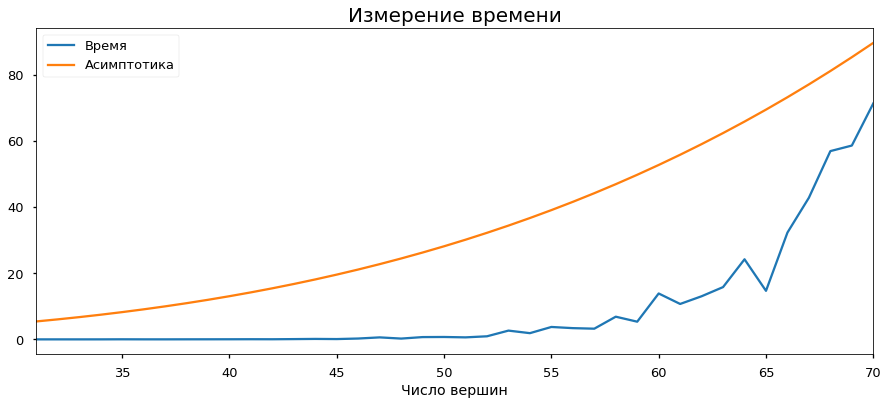
\includegraphics[width=\linewidth]{plot.png}
    \caption{Время работы}
\end{figure}

В роли асимтотики выступает функция $0.00004 \cdot n^2 3^{n / 3}$

\newpage
\tableofcontents

\newpage
\bibliographystyle{unsrt}%Used BibTeX style is unsrt
\bibliography{biblio}

\end{document}

%https://www.ics.uci.edu/~eppstein/pubs/BeiEpp-DIMACS-00.pdf